\documentclass[14pt]{article}
\usepackage[utf8]{inputenc}
\usepackage[T2A]{fontenc}
\usepackage[russian]{babel} % Кириллица uchun, lekin matn lotin yozuvida
\usepackage{amsmath, amssymb}
\usepackage{geometry}
\usepackage{graphicx}
\usepackage{xcolor}
\usepackage{hyperref}
\usepackage{tasks}
\usepackage{tcolorbox}
\tcbuselibrary{skins, breakable, theorems}
\usepackage{fancyhdr}
\usepackage{lastpage}
\usepackage{enumitem}
\usepackage{paracol}
\usepackage{ifthen}
\usepackage{needspace}

% Определение команд для тангенса и котангенса (русский стиль)
\newcommand{\tg}{\operatorname{tg}}
\newcommand{\ctg}{\operatorname{ctg}}

% Настройка геометрии
\geometry{a4paper, left=10mm, right=10mm, top=20mm, bottom=20mm, headheight=15pt}

% Цветовая палитра
\definecolor{primary}{RGB}{52, 152, 219}
\definecolor{secondary}{RGB}{46, 204, 113}
\definecolor{accent}{RGB}{155, 89, 182}
\definecolor{lightbg}{RGB}{248, 249, 250}
\definecolor{taskborder}{RGB}{230, 230, 230}
\definecolor{optionbg}{RGB}{240, 242, 245}

% Основной фон страницы
\pagecolor{lightbg}

% Настройка гиперссылок
\hypersetup{
    colorlinks=true,
    linkcolor=primary,
    urlcolor=primary,
}

% Колонтитулы
\pagestyle{fancy}
\fancyhf{}
\fancyhead[L]{\textcolor{primary}{\textbf{MathCore | MOCK Test-7}}}
\fancyhead[R]{\textcolor{secondary}{Abdunazarov M.X.}}
\fancyfoot[L]{\href{https://t.me/Math_Core_Dtm_MS_Att}{\textcolor{primary}{MathCore}}}
\fancyfoot[R]{\href{https://t.me/Abd_mardon}{\textcolor{secondary}{@Abd\_mardon}}}
\fancyfoot[C]{\textcolor{gray}{\thepage/\pageref{LastPage}}}
\renewcommand{\headrulewidth}{0.5pt}
\renewcommand{\headrule}{\hbox to\headwidth{\color{primary}\leaders\hrule height \headrulewidth\hfill}}
\renewcommand{\footrulewidth}{0.5pt}
\renewcommand{\footrule}{\hbox to\headwidth{\color{secondary}\leaders\hrule height \footrulewidth\hfill}}

% Титульная страница
\title{\Huge \textbf{\textcolor{primary}{MOCK Test-7}}}
\author{\textcolor{secondary}{Abdunazarov M.X.}}
\date{}

% Стиль для карточки вопроса
\newtcolorbox{questionbox}[2][]{
    enhanced,
    breakable,
    colback=white,
    colframe=primary,
    coltitle=white,
    fonttitle=\bfseries\large,
    title={Masala \hfill \textcolor{white}{#2}},
    attach boxed title to top left={xshift=5mm, yshift=-2mm},
    boxed title style={size=small, colback=primary, sharp corners},
    sharp corners,
    boxrule=0.5pt,
    left=5mm,
    right=5mm,
    top=5mm,
    bottom=5mm,
    drop fuzzy shadow,
    #1
}

% Стиль для вариантов ответов
\newlist{options}{enumerate}{1}
\setlist[options]{
    label=\textbf{\Alph*)},
    leftmargin=*,
    itemsep=2pt,
    topsep=5pt,
    before={\vspace{2mm}\begin{tcolorbox}[
        colback=optionbg,
        colframe=white,
        sharp corners,
        boxrule=0pt,
        left=2mm,
        right=2mm,
        top=2mm,
        bottom=2mm,
    ]},
    after={\end{tcolorbox}\vspace{2mm}},
}

% Для рисунков
\newcommand{\questionimage}[2][0.5\linewidth]{%
    \begin{center}
        \includegraphics[width=#1]{#2}
    \end{center}
}

% Для удобства: команда вставки вопроса с рисунком
\newcommand{\questionitem}[4]{%
    \needspace{5cm}
    \begin{questionbox}{#1}
        #2
        \ifx&#3&%
        \else
            \questionimage{#3}
        \fi
        \begin{options}
            #4
        \end{options}
    \end{questionbox}
}

\begin{document}

% Титульная страница
\maketitle
\begin{center}
    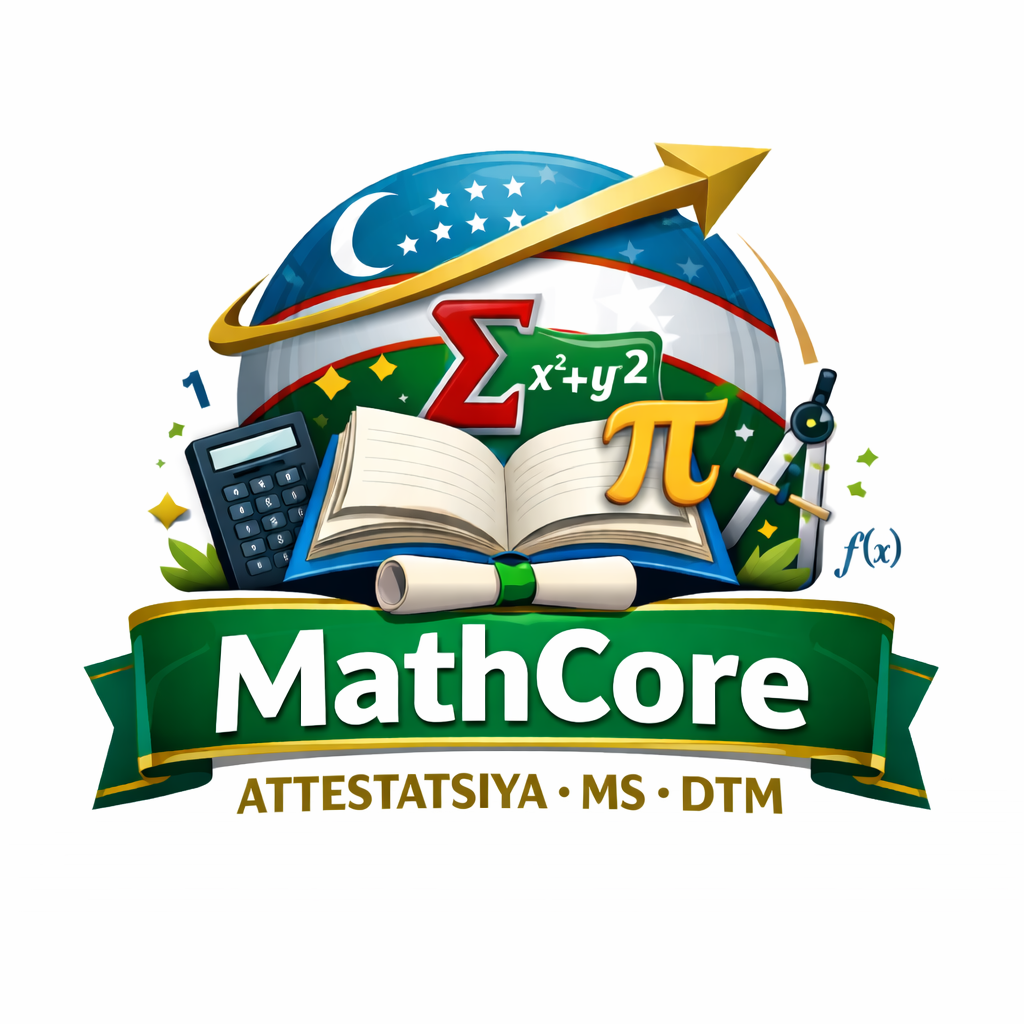
\includegraphics[width=0.2\textwidth]{logo.png} \\[5mm]
    \textcolor{gray}{\small Telegram: \href{https://t.me/Math_Core_Dtm_MS_Att}{@Math\_Core\_Dtm\_MS\_Att}}
\end{center}
\vspace{5mm}

% Masala 1
\begin{questionbox}{1}
    Agar \(f(x)\) kamayuvchi funksiya, \(g(x)\) o'suvchi funksiya va \(x_1 < x_2 < x_3 < x_4\) bo'lsa,
    \(f(x_1) - f(x_2) = a\), \(g(x_3) - g(x_4) = b\) bo'lsa, quyidagi tasdiqlardan qaysi biri to'g'ri?
    \begin{options}
        \item \(a \cdot b > 0\)
        \item \(a + b < 0\)
        \item \(-a + b > 0\)
        \item \(a > 0 > b\)
    \end{options}
\end{questionbox}

% Masala 2
\begin{questionbox}{2}
    Agar \(5 + 6 + 7 + 8 + 9 + \cdots + n = 290\) bo'lsa, \(n = ?\)
    \begin{options}
        \item 36
        \item 24
        \item 32
        \item 28
    \end{options}
\end{questionbox}

% Masala 3
\begin{questionbox}{3}
    Ikki xonali \(x\) soni uchun \(\text{EKUB}(x, 13) = 1\) bajariladi. \(x\) sonining raqamlari ko'paytmasining maksimal qiymatini toping.
    \begin{options}
        \item 81
        \item 69
        \item 75
        \item 85
    \end{options}
\end{questionbox}

% Masala 4
\begin{questionbox}{4}
    \(7 \cdot 7^{15}\) ni 8 ga bo'lgandagi qoldiqni toping.
    \begin{options}
        \item 1
        \item 7
        \item 3
        \item 6
    \end{options}
\end{questionbox}

% Masala 5
\begin{questionbox}{5}
    \(m\) ning qanday qiymatida \(x(x + a)(x + b)(x + a + b) + 25m^2\) ifoda to'liq kvadrat bo'ladi?
    \begin{options}
        \item \(\pm \frac{ab}{5}\)
        \item \(\pm \frac{ab}{10}\)
        \item \(\pm ab\)
        \item \(\pm \frac{ab}{4}\)
    \end{options}
\end{questionbox}

% Masala 6
\begin{questionbox}{6}
    Agar \(x^2 - x = 3\) bo'lsa, \(\frac{x^2 -3}{x^2+x-3}\) ifodaning qiymatini toping.
    \begin{options}
        \item \(-\frac{1}{2}\)
        \item \(-\frac{1}{3}\)
        \item \(1\)
        \item \(\frac{1}{2}\)
    \end{options}
\end{questionbox}

% Masala 7
\begin{questionbox}{7}
    \(x^{\lg^2 x - 3\lg x + 1} < 1000\) tengsizlikni yeching.
    \begin{options}
        \item \((0; 100)\)
        \item \((0; 1000)\)
        \item \((10; 100)\)
        \item \((100; 1000)\)
    \end{options}
\end{questionbox}

% Masala 8
\begin{questionbox}{8}
    6 ta haddan iborat geometrik progressiyada dastlabki uch hadi yig'indisi 26 ga, oxirgi uch hadi yig'indisi 702 ga teng. Progressiyaning maxrajini toping.
    \begin{options}
        \item 8
        \item 6
        \item 2
        \item 3
    \end{options}
\end{questionbox}

% Masala 9
\begin{questionbox}{9}
    \(3\sqrt{5-x} \le (x-4)\ln(x-4)\) tengsizlikni nechta butun son qanoatlantiradi?
    \begin{options}
        \item \(\varnothing\)
        \item 2
        \item 1
        \item 3
    \end{options}
\end{questionbox}

% Masala 10
\begin{questionbox}{10}
    \([0; 2\pi]\) oralig'ida \(\left(x - \frac{\pi}{6}\right)\left(\sin x - \frac{1}{2}\right) > 0\) tengsizlikning yechimlarini toping.
    \begin{options}
        \item \(\left[0; \frac{\pi}{6}\right]\)
        \item \(\left(\frac{\pi}{6}; \frac{5\pi}{6}\right)\)
        \item \(\left(\frac{\pi}{6}; \frac{\pi}{3}\right)\)
        \item \(\left(0; \frac{\pi}{6}\right) \cup \left(\frac{\pi}{6}; \frac{5\pi}{6}\right)\)
    \end{options}
\end{questionbox}

% Masala 11
\begin{questionbox}{11}
    \(\arctg 1 + \arctg 2 + \arctg 3\) ni hisoblang.
    \begin{options}
        \item \(\frac{\pi}{2}\)
        \item \(\pi\)
        \item \(\frac{3\pi}{2}\)
        \item \(2\pi\)
    \end{options}
\end{questionbox}

% Masala 12
\begin{questionbox}{12}
    Kutubxonada 4 xil kitob mavjud bo'lib, har bir turdagi kitoblar yetarli miqdorda. 5 ta kitobni necha usulda tanlash mumkin?
    \begin{options}
        \item \(56\)
        \item \(4^5\)
        \item \(5^4\)
        \item 20
    \end{options}
\end{questionbox}

% Masala 13
\begin{questionbox}{13}
    Tanga 5 marta tashlanadi. Tanganing pullik tomoni bilan 3 marta tushish ehtimolini toping.
    \begin{options}
        \item \(\frac{5}{32}\)
        \item \(\frac{5}{16}\)
        \item \(\frac{7}{32}\)
        \item \(\frac{1}{32}\)
    \end{options}
\end{questionbox}

% Masala 14
\begin{questionbox}{14}
    \((x^3 + \frac{1}{\sqrt{x}})^{14}\) ifodaning ozod hadini toping.
    \begin{options}
        \item 50
        \item 45
        \item 91
        \item 84
    \end{options}
\end{questionbox}

% Masala 15
\begin{questionbox}{15}
    Qutida 1 dan 10 gacha raqamlangan 10 ta shar bor. Qutidan tasodifiy ravishda ikkita shar tanlanadi. Tanlangan sharlar raqamlari yig'indisi 14 ga tengligi ma'lum. 6 raqamli shar tanlanganlik ehtimoli qanday?
    \begin{options}
        \item \(\frac{1}{3}\)
        \item \(\frac{1}{6}\)
        \item \(\frac{1}{2}\)
        \item \(\frac{2}{3}\)
        \item \(\frac{5}{6}\)
    \end{options}
\end{questionbox}

% Masala 16
\begin{questionbox}{16}
    \(h(x) = \frac{f(3x)}{g(2x)}\) funksiyasi berilgan. \(f(3) = 2\), \(g(2) = 3\), \(f'(3) = 4\) va \(g'(2) = 5\) ekanligi ma'lum bo'lsa , \(h'(1)\) ni toping.
    \begin{options}
        \item \(\frac{9}{16}\)
        \item \(\frac{2}{3}\)
        \item \(\frac{16}{9}\)
        \item \(\frac{3}{4}\)
    \end{options}
\end{questionbox}

% Masala 17
\begin{questionbox}{17}
    Rasmda \(y = x^3\) funksiyasining grafigi tasvirlangan. \(x=1\) nuqta bu funksiyaga tegishli. Bo'yalgan soha yuzini toping.
   \begin{center}
       \centering
       
\includegraphics[width=0.4\linewidth]{1.png}
   \end{center}
    \begin{options}
        \item \(\frac{3}{2}\)
        \item \(\frac{1}{3}\)
        \item \(\frac{1}{6}\)
        \item \(\frac{1}{2}\)
    \end{options}
\end{questionbox}

% Masala 18
\begin{questionbox}{18}
    \(\displaystyle \int \tg^2 x \, dx + \int \tg^4 x \, dx\) integralini hisoblang.
    \begin{options}
        \item \(\frac{1}{3} \tg^2 x + C\)
        \item \(x + 3\tg^2 x + C\)
        \item \(3x + \tg x + C\)
        \item \(\frac{1}{3} \tg^3 x + C\)
    \end{options}
\end{questionbox}

% Masala 19
\begin{questionbox}{19}
    Agar \(f(x+2) = f(x) + x\) va \(f(2) = 3\) bo'lsa, \(f(8)\) ni toping.
    \begin{options}
        \item 15
        \item 9
        \item 12
        \item 10
    \end{options}
\end{questionbox}

% Masala 20
\begin{questionbox}{20}
    \(\displaystyle \int_{-1}^{0} \frac{e^{2x} - 2}{e^x} \, dx\) ni hisoblang.
    \begin{options}
        \item \(2e - \frac{1}{e}\)
        \item \(2e + 3\)
        \item \(2e + \frac{1}{e} - 3\)
        \item \(\frac{3e - 2e^2 - 1}{e}\)
    \end{options}
\end{questionbox}

% Masala 21
\begin{questionbox}{21}
    Berilgan ma'lumotlardan foydalanib, bo'yalgan soha yuzini toping.
    \begin{center}
        \begin{center}
            \centering
            
\includegraphics[width=0.3\linewidth]{2.png}
        \end{center}
    \end{center}
    \begin{options}
        \item \(\frac{14}{3}\)
        \item \(\frac{16}{3}\)
        \item \(\frac{10}{2}\)
        \item \(\frac{17}{3}\)
    \end{options}
\end{questionbox}

% Masala 22
\begin{questionbox}{22}
    Quyidagi tasdiqlardan nechtasi noto'g'ri?
    \begin{enumerate}[label=\arabic*.]
        \item Agar uchburchak tomonlari 4, 6 va 9 ga teng bo'lsa, uning perimetri 19 ga teng;
        \item Agar ikki to'g'ri chiziq uchinchi to'g'ri chiziq bilan kesilganda ichki almashinuvchi burchaklar teng bo'lsa, bu to'g'ri chiziqlar paralleldir;
        \item Uchburchakka ichki chizilgan aylana markazi uning bissektrisalari kesishgan nuqtada yotadi;
        \item Ixtiyoriy muntazam ko'pburchakka ichki chizilgan aylana radiusi \(R = \dfrac{a}{2 \sin \frac{180^\circ}{n}}\) ga teng (bu yerda \(a\) — ko'pburchak tomoni, \(n\) — tomonlar soni).
    \end{enumerate}
    \begin{options}
        \item 1
        \item 3
        \item 2
        \item 4
    \end{options}
\end{questionbox}

% Masala 23
\begin{questionbox}{23}
    Trapetsiyada diagonallar kesishganda uchburchaklar hosil bo'ldi. Ma'lumki, \(S_{\triangle AED} = 8\) va \(S_{\triangle DEC} = 4\). Bo'yalgan soha yuzini toping.
    \begin{center}
       
\includegraphics[width=0.3\linewidth]{3.png}
    \end{center}
    \begin{options}
         \item 24
        \item 12
        \item 16
        \item 14
    \end{options}
\end{questionbox}

% Masala 24
\begin{questionbox}{24}
    Uchburchak tomonlari uchlaridan boshlab \(3:5:7\) nisbatda bo'lindi. Bo'lish nuqtalari orqali asosga parallel to'g'ri chiziqlar o'tkazildi. Hosil bo'lgan shakllar yuzlarining nisbatini toping.
    \begin{options}
        \item \(3: 5: 7\)
        \item \(9: 25: 49\)
        \item \(9: 64: 225\)
        \item \(9: 55: 161\)
    \end{options}
\end{questionbox}

% Masala 25
\begin{questionbox}{25}
    Rasmda ABC va ADC to'g'ri burchakli uchburchaklar berilgan (DE \(\perp\) AC). Berilgan ma'lumotlardan foydalanib, x ni toping.
    \begin{center}
        
\includegraphics[width=0.3\linewidth]{4.png}
    \end{center}
    \begin{options}
        \item \(16\)
        \item \(20\)
        \item \(8\sqrt{2}\)
        \item \(16\sqrt{2}\)
    \end{options}
\end{questionbox}

% Masala 26
\begin{questionbox}{26}
   \(S_1 - S_2\) qiymatini toping.
   \begin{center}
       \centering
       
\includegraphics[width=0.3\linewidth]{5.png}
   \end{center}
    \begin{options}
        \item \(2\pi\)
        \item \(4\pi\)
        \item \(3\pi\)
        \item \(6\pi\)
    \end{options}
\end{questionbox}

% Masala 27
\begin{questionbox}{27}
    \(\overrightarrow{AB}(3; 5; -7)\) va \(\overrightarrow{AD}(-11; 7; 3)\) vektorlari bilan ABCD parallelogrammi berilgan. O — parallelogramm diagonallarining kesishish nuqtasi. \(\overrightarrow{OD}\) vektori koordinatalari yig'indisini toping.
    \begin{options}
        \item 1
        \item 0
        \item -1
        \item 2
    \end{options}
\end{questionbox}

% Masala 28
\begin{questionbox}{28}
    Rasmdagi ABCD to'g'ri to'rtburchakda \(S_{\triangle AOD}=30\) va \(S_{\triangle BOC}=50\) va \(DC=16\). AD tomon uzunligini toping.
    \begin{center}
        
\includegraphics[width=0.3\linewidth]{6.png}
    \end{center}
    \begin{options}
        \item 10
        \item 45
        \item 15
        \item 40
    \end{options}
\end{questionbox}

% Masala 29
\begin{questionbox}{29}
    Markazi O nuqtada bo'lgan yarim aylanaga D nuqtada urinma o'tkazilgan. Berilgan ma'lumotlarga asoslanib, OD ni toping.
    \begin{center}
         
\includegraphics[width=0.5\linewidth]{7.png}
    \end{center}
    \begin{options}
        \item 2
        \item 6
        \item 4
        \item 3
    \end{options}
\end{questionbox}

% Masala 30
\begin{questionbox}{30}
    Rasmda qirrasi 1 ga teng kublar tasvirlangan. Nuqta chiziq bilan belgilangan chiziq bo'ylab uzunlik nechaga teng?
    \begin{center}
         
\includegraphics[width=0.5\linewidth]{8.png}
    \end{center}
    \begin{options}
        \item \(\sqrt{13}\)
        \item \(\sqrt{12}\)
        \item \(\sqrt{14}\)
        \item \(\sqrt{17}\)
    \end{options}
\end{questionbox}

% Masala 31
\begin{questionbox}{31}
    \(K(0, 7)\) va \(L(1, 0)\) nuqtalari berilgan. KL kesmani Oy o'qi atrofida \(90^\circ\) ga aylantirishdan hosil bo'lgan jismning hajmini toping.
    \begin{center}
        \centering
        
\includegraphics[width=0.3\linewidth]{9.png}
    \end{center}
    \begin{options}
        \item \(\frac{7\pi}{6}\)
        \item \(\frac{7\pi}{3}\)
        \item \(\frac{7\pi}{12}\)
        \item \(\frac{9\pi}{4}\)
    \end{options}
\end{questionbox}

% Masala 32
\begin{questionbox}{32}
    \(x\) o'qi va \(x-y+4=0\) hamda \(x-2y+8=0\) chiziqlari bilan chegaralangan sohani \(y\) o'qi atrofida 360° ga aylantirishdan hosil bo'lgan jismning hajmi nechaga teng?
    \begin{options}
        \item \(32\pi\)
        \item \(48\pi\)
        \item \(54\pi\)
        \item \(64\pi\)
    \end{options}
\end{questionbox}

% Masala 33
\begin{questionbox}{33}
    Agar \(AD=22\), \(BE=16\), \(EF=12\) va \(KF=7\) bo'lsa, \(PL\) kesma uzunligini toping.
    \begin{center}
        
\includegraphics[width=0.3\linewidth]{12.png}
    \end{center}
    \begin{options}
        \item 26
        \item 30
        \item 25
        \item 27
    \end{options}
\end{questionbox}

% Masala 34
\begin{questionbox}{34}
    To'g'ri burchakli uchburchakning gipotenuzasi 12 ga teng. Uchburchakning barcha uchlaridan 10 masofada joylashgan va uning tekisligidan tashqarida nuqta berilgan. Bu nuqtadan uchburchak tekisligigacha bo'lgan masofani toping.
    \begin{options}
        \item 8
        \item 10
        \item \(\sqrt{44}\)
        \item 12
    \end{options}
\end{questionbox}

% Masala 35
\begin{questionbox}{35}
    Konusning hajmi \(3\pi\) m\(^3\) ga teng. Agar uning yon sirti yoyilmasi yarim doira bo'lsa, konusning to'la sirti yuzini toping.
    \begin{options}
        \item \(6\pi\)
        \item \(2\pi\)
        \item \(9\pi\)
        \item \(18\pi\)
    \end{options}
\end{questionbox}

\end{document}